\title{Computational Science and Engineering:\\Parallele Lastbalancierung mit Octrees}
\author {
	Maximilian Knespel
	\newline	\newline
	Betreuer: \and Nico Hoffmann
}
\date{}
%\date{7. Juli 2016}


\begin{document}

\begin{frame}
	\titlepage
\end{frame}

%\begin{frame}
%	\frametitle{Outline}
%	\setcounter{tocdepth}{1}
%	\tableofcontents
%\end{frame}


%%%%%%%%%%%%%%%%%%%%%%%%%%%%%%%%%%%%%%%%%%%%%%%%%%%%%%%%%%%%%%%%%%%%%%%%%%%%%%%%
\section{Einführung}
%%%%%%%%%%%%%%%%%%%%%%%%%%%%%%%%%%%%%%%%%%%%%%%%%%%%%%%%%%%%%%%%%%%%%%%%%%%%%%%%

% Was ist das Ziel der Arbeit/des Vortrags
%   Verfügbarmachen von
% Übersicht des Vortrags


%%%%%%%%%%%%%%%%%%%%%%%%%%%%%%%%%%%%%%%%%%%%%%%%%%%%%%%%%%%%%%%%%%%%%%%%%%%%%%%%
\section{Spark}
%%%%%%%%%%%%%%%%%%%%%%%%%%%%%%%%%%%%%%%%%%%%%%%%%%%%%%%%%%%%%%%%%%%%%%%%%%%%%%%%

% Following:
%  - https://www.toptal.com/spark/introduction-to-apache-spark
%  - "Learning Spark"

\begin{frame}
MapReduce Paper Google:
 -
Hadoop: Core MapReduce + verteiltes Dateisystem(HDFS,NFS,...)

% Sagen:
%  - 2009 als Forschungsprojekt am UC Berkely Lab angefangen
%  - 2013 Transfer zur Apache Software Foundation
Nachfolger zu Hadoop MapReduce. Geschrieben in Scala.
Vorteile gegenüber von Hadoop MapReduce:
  + Kann in-memory arbeiten, was Hadoop nicht anbot
  + komplexere Funktionen auch on-disk schneller als Hadoop!
  + interaktive Konsole zum schnellen Prototyping
  + Stellt viele Komplexbefehle zur Verfügung
    % vereinfachtere Programmierung gegenüber simplen MapReduce
    %   -> siehe nächste Folie
  + hohe Anwendbarkeit: Aus vielen Sprachen heraus nutzbar: Scala, Java, Python, SQL.
  + Im Gegensatz zu zu Hadoop MapReduce auch lokales Dateisystem nutzbar (Hadoop erzwingt HDFS)
\end{frame}


\begin{frame}
    Ermittlung der häufigsten Wörter in einem Text:

    \begin{lstlisting}[language=java]   % scala
        sc.
          textFile("./*").
          flatMap( line => line.split(" ") ).
          map( word => (word, 1) ).
          reduceByKey( (a, b) => a + b ).
          sortBy( _._2, false /*descending*/ ).
          take(500).
          foreach( println )
    \end{lstlisting}

    % Vergleich Hadoop MapReduce word count:
    %   https://hadoop.apache.org/docs/current/hadoop-mapreduce-client/hadoop-mapreduce-client-core/MapReduceTutorial.html#Example:_WordCount_v1.0
    % https://hadooptutorial.wikispaces.com/Sorting+feature+of+MapReduce
    % mit Spark version:
    %

    % Top 4:
    %  (ich,57766)
    %  (die,47869)
    %  (und,47663)
    %  (das,38866)
\end{frame}

\begin{frame}
GraySort Gewinner 5.11.2014: Apache Spark von Reynold Xin (Databricks Inc.)
  % https://databricks.com/blog/2014/10/10/spark-petabyte-sort.html
  %  https://databricks.com/blog/2014/11/05/spark-officially-sets-a-new-record-in-large-scale-sorting.html
  % Sagen:
  %  - nur kurzzeitig, abgelöst von TritonSort, aktuell FuxiSort:
  %     - (Alibaba Cloud Computing Inc) mittels Apsara(distributed FS Pangu + distribution computation framework Fuxi, written in C/C++)
  %  - 206 nodes a 32 virtuelle cores (Amazon Elastic Compute Cloud - EC2) vs. HadoopRecord 2100 nodes a 24 cores (physisch)
  %  - GraySort sortiert mindestens 100TB, das heißt auf große Daten ausgelegt
  - \begin{tabular}{c|c}
    Apache Spark                &   Hadoop               \\
    \hline
    \SI{100}{\tera\byte}        & \SI{102.5}{\tera\byte} \\
    \SI{1406}{\second}          & \SI{4238}{\second}     \\
    207 Amazon EC2 i2.8xlarge Nodes
      - 32 vCores (2.5Ghz Intel Xeon E5-2670 v2) % 8 cores, 16 SMT
      - 244GB memory
      - 8 \times \SI{800}{\giga\byte} SSD
    Summe: \SI{1324.8}{\tera\byte} mit \SI{618}{\giga\byte\per\second}
    &
    2100 Nodes
      - 2 \times \SI{2.3}{\giga\hertz} hexcore Xeon E5-2630
      - 64 GB RAM
      - 12 \times \SI{3}{\tera\byte} disks
    Summe: \SI{75600}{\tera\byte} mit \approx \SI{3150}{\giga\byte\per\second} Durchsatz
  % http://sortbenchmark.org/
  % https://databricks.com/blog/2014/11/05/spark-officially-sets-a-new-record-in-large-scale-sorting.html
  => 3x schneller bei 1/10 Knoten und 1/5 Datendurchsatz
  % Sagen:
  %     Autoren ahbena uch erste Sortierung mit 1 Petabyte an Daten auf einen öffentlcihen cloud damit gemacht. (16h 3800 nodes)
\end{frame}

% Was ist Spark, warum will ich es nehmen
% Wie funktioniert Spark ( RDD, Reduce, Slurm )
% Ein Beispiel mit Spark ( Monte Carlo und/oder word count -> chat log :) )


% \begin{frame}
% \begin{lstlisting}[language=bash]
% jobid=$(sbatch "$@" --output="$SPARK_LOGS/%j.out" --error="$SPARK_LOGS/%j.err" $HOME/scaromare/start_spark_slurm.sh)
% jobid=${jobid##Submitted batch job }
%
%
% function startSpark() {
%     export SPARK_LOGS=$HOME/spark/logs
%     mkdir -p "$SPARK_LOGS"
%     if [ ! -d "$SPARK_LOGS" ]; then return 1; fi
%     jobid=$(sbatch "$@" --output="$SPARK_LOGS/%j.out" --error="$SPARK_LOGS/%j.err" $HOME/scaromare/start_spark_slurm.sh)
%     jobid=${jobid##Submitted batch job }
%     echo "Job ID : $jobid"
%     # looks like: 16/05/13 20:44:59 INFO MasterWebUI: Started MasterWebUI at http://172.24.36.19:8080
%     echo -n "Waiting for Job to run and Spark to start.."
%     MASTER_WEBUI=''
%     while [ -z "$MASTER_WEBUI" ]; do
%         echo -n "."
%         sleep 1s
%         if [ -f $HOME/spark/logs/$jobid.err ]; then
%             MASTER_WEBUI=$(sed -nE 's|.*Started MasterWebUI at (http://[0-9.:]*)|\1|p' $HOME/spark/logs/$jobid.err)
%         fi
%     done
%     echo "OK"
%     export MASTER_WEBUI
%     export MASTER_ADDRESS=$(cat ~/spark/logs/${jobid}_spark_master)
%     function sparkSubmit() {
%         ~/spark-1.5.2-bin-hadoop2.6/bin/spark-submit --master $MASTER_ADDRESS $@
%     }
%     cat "$SPARK_LOGS"/$jobid.*
%     echo "MASTER_WEBUI   : $MASTER_WEBUI"
%     echo "MASTER_ADDRESS : $MASTER_ADDRESS"
% }
% export -f startSpark
%
% \end{frame}

startSpark --time=04:00:00 --nodes=$((nodes+1)) --partition=gpu2 --gres=gpu:$gpusPerNode --cpus-per-task=$coresPerNode
sparkSubmit ~/scaromare/MontePi/singleNode/singleGpu/multiGpuTestSpark/MontePi.jar \
                 $((nPerSlice*nSlices)) $nSlices $gpusPerNode 2>/dev/null |
                 tee tmp.log | tee -a "$fname-gpu.log"



%%%%%%%%%%%%%%%%%%%%%%%%%%%%%%%%%%%%%%%%%%%%%%%%%%%%%%%%%%%%%%%%%%%%%%%%%%%%%%%%
\section{Rootbeer}
%%%%%%%%%%%%%%%%%%%%%%%%%%%%%%%%%%%%%%%%%%%%%%%%%%%%%%%%%%%%%%%%%%%%%%%%%%%%%%%%

\begin{frame}
% sagen:
%  - Leider wurde die meiste Bearbeitungszeit für diesen Beleg vom Lösen von Bugs beansprucht, sodass ich nicht darauf verzichten kann, zumindest einige davon zu erwähnen, auf dass sie jemanden helfen mögen, der einen ähnlichen Ansatz wie ich verfolgen möchte
Rootbeer zu beachten:
  - Bei dem Versuch Rootbeer mit Java 8 zu benutzen, kommt es zu
        java.lang.NullPointerException
            at soot.rbclassload.RootbeerClassLoader.loadHierarchySootClasses(RootbeerClassLoader.java:963)
    Nur Java 6 ist offiziell unterstützt, aber Java 7 scheint auch zu funktionieren
    % https://github.com/pcpratts/rootbeer1/issues/175 - Issues with jre1.8
  - GCC 4.9 nur unterstützt (wegen CUDA-Compiler)
  - Kaum neue Commits auf Github seit Juni 2015
    % https://github.com/pcpratts/rootbeer1/commits/master
  - Die option '-computecapability=sm_30' ist Pflicht, da seit CUDA 7.0 die Standardarchitektur "compute_12" nicht mehr unterstützt wird (korrekt nun "sm_12")
        nvcc fatal   : Unsupported gpu architecture 'compute_12'
    % https://github.com/pcpratts/rootbeer1/issues/180 - CUDA 7.0: nvcc fatal: Unsupported gpu architecture 'compute_12'
  - Automatische Kernel-Konfiguration hat einen Bug, der standardmäßig immer so viele Kernel startet wie gleichzeitig auf einem Shared Multiprozessor laufen können.
    % return new ThreadConfig( block_shaper.getMaxThreadsPerBlock(), 1, 1,
    %                          block_shaper.getMaxBlocksPerProc(), 1,
    % https://github.com/pcpratts/rootbeer1/issues/168
  - Bug wo Rootbeer hat standardmäßig versucht den gesamten freien Speicher minus den benötigten zu alloziieren versuchte
    % sagen:
    %  - verhinderte multi-GPU, weil ein Kontext schon so gut wie den gesamten Speicher für sich beanspruchen wollte.
    %  - nur ein Problem mit multiple Rootbeer.jar
    % https://github.com/mxmlnkn/rootbeer1/commit/0d9699a40b06a7e5efee7213ca7fb215d6ef1377
    % https://github.com/mxmlnkn/rootbeer1/commit/cc2318673077a52f13a8c4b4d294fbd39e639ca5
    % /media/d/Studium/9TH SEMESTER/scaromare/MontePi/multiNode/multiGpu/scala$ /opt/spark-1.5.2/bin/spark-submit --master local[4] --class TestMonteCarloPi MontePi.jar 268435456 2
    %   16/01/22 03:27:59 ERROR Executor: Exception in task 1.0 in stage 0.0 (TID 1)
    %rg.trifort.rootbeer.runtime.CudaErrorException: CUDA_ERROR_OUT_OF_MEMORY: Error in cuMemAlloc: gpu_object_mem
    %   at org.trifort.rootbeer.runtime.CUDAContext.nativeBuildState(Native Method)
    %   at org.trifort.rootbeer.runtime.CUDAContext.access$1100(CUDAContext.java:17)
    %   at org.trifort.rootbeer.runtime.CUDAContext$GpuEventHandler.onEvent(CUDAContext.java:315)
    %   at org.trifort.rootbeer.runtime.CUDAContext$GpuEventHandler.onEvent(CUDAContext.java:308)
    %   at com.lmax.disruptor.BatchEventProcessor.run(BatchEventProcessor.java:128)
    %   at java.util.concurrent.ThreadPoolExecutor.runWorker(ThreadPoolExecutor.java:1145)
    %   at java.util.concurrent.ThreadPoolExecutor$Worker.run(ThreadPoolExecutor.java:615)
    %   at java.lang.Thread.run(Thread.java:745)
  - die ausführbare jar für Spark darf kein Leerzeichen im Pfad enthalten:
    % $SPARK_ROOT/bin/spark-submit --master $MASTER_ADDRESS ./src/sort.py "$(pwd)"/data/The_Complete_Works_of_Willia.txt
    %   java.io.FileNotFoundException: Added file file:/media/f/Studium/9TH%20SEMESTER/scaromare/spark-gpu/src/sort.py does not exist.
    %      at org.apache.spark.SparkContext.addFile(SparkContext.scala:1365)
%  - Alignement Bug in Speicherserialisierung
%       https://github.com/mxmlnkn/rootbeer1/commit/cc2318673077a52f13a8c4b4d294fbd39e639ca5
  - Zu kompilierende jar an Rootbeer >muss< auf .jar enden
    % normalerweise sollte die Dateiendung unter Linux egal sein, gibt Magic Bytes und Co
    % #Warning: the following soot-classpath entry is not a supported archive file (must be .zip, .jar or .apk): MontePiGPU.jar.tmp
\end{frame}

\begin{frame}
Scala GPU:
  - ScalaCL ( "ScalaCL is not production-ready!" )
  - BIDMach
  - Firepile
  - Rootbeer (
\end{frame}

\begin{frame}
Run on Taurus:
    module load java/jdk1.7.0_25 scala/2.10.4 cuda/7.0.28
    # manuelle Installation von maven, ant, spark, zipmerge
    % für spark wurden precompiled binaries genommen, weil es bei der Kompilation auch Probleme gab, die nicht behoben werden konnten
    export PATH="$PATH:$HOME/spark-1.5.2-bin-hadoop2.6/bin/:$HOME/spark-1.5.2-bin-hadoop2.6/sbin/:$HOME/programs/bin"
\end{frame}

\begin{frame}
    \frametitle{Rootbeer Funktionsweise}
    3.) Rootbeer constructor
    3.1.) CUDALoader constructor
    3.2.) CUDALoader.load
          Load shared libraries with fixed absolute paths mostly ...
              m_libCudas.add("/usr/lib64/libcuda.so");
              m_libCudas.add("/usr/lib/x86_64-linux-gnu/libcudart.so.5.0");
              m_rootbeerRuntimes.add(RootbeerPaths.v().getRootbeerHome()+"rootbeer_x64.so.1");
              m_rootbeerCudas.add(RootbeerPaths.v().getRootbeerHome()+"rootbeer_cuda_x64.so.1");
    4.) Rootbeer.getDevices
          Class c = Class.forName("org.trifort.rootbeer.runtime.CUDARuntime");
          Constructor<IRuntime> ctor = c.getConstructor();
          m_cudaRuntime = ctor.newInstance();
          m_cards.addAll( m_cudaRuntime.getGpuDevices() );
    4.1.) CUDA_Runtime.c
            status = cuDeviceGet(&device, i);
            cuDeviceGetAttribute(...)
            [...]
    5.) GPUDevice.createContext -> CUDAContext -> native initializeDriver
            https://de.wikipedia.org/wiki/Java_Native_Interface
        ./csrc/org/trifort/rootbeer/runtime/CUDAContext.c:JNIEXPORT void JNICALL Java_org_trifort_rootbeer_runtime_CUDAContext_initializeDriver
            only saves function pointers to context.java
    6.) Rootber.run
    6.1.) Context context = createDefaultContext(); // skipped for multi-GPU
    6.2.) context.setThreadConfig(thread_config);
    6.3.) context.setKernel(work.get(0));
    6.4.) context.setUsingHandles(true);
    6.5.) context.buildState();
            gpuEvent.setValue(GpuEventCommand.NATIVE_BUILD_STATE);
                GpuEventHandler.onEvent
                    nativeBuildState( ..., gpuDevice.getDeviceId(), ... )
                        Java_org_trifort_rootbeer_runtime_CUDAContext_nativeBuildState in CUDAContext.c
    6.6.) context.run(work)
            context.runAsync(work)
                gpuEvent.setValue(GpuEventCommand.NATIVE_RUN_LIST);
                    GpuEventHandler.onEvent
                        writeBlocksTemplate();
                        runGpu();
                            cudaRun(nativeContext, objectMemory, b2i(!usingHandles), stats);
                        readBlocksTemplate();
          private native void cudaRun(long nativeContext, Memory objectMem, int usingKernelTemplates, StatsRow stats);

Rootbeer-Paper:
        1) serialize state to GPU memory
        2) define the kernel code that the GPU will execute
        3) control the kernel
        4) deserialize state back to CPU memory
      -> "serialize"?
      => Rootbeer does these things automatically in contrast to CUDA- and OpenCL- Java language bindings
      supports:
        1) single and multi-dimensional arrays of primitive and reference types
        2) composite objects
        3) instance and static fields
        4) dynamic memory allocation
        5) inner classes
        6) synchronized methods and monitors
        7) strings
        8) exceptions that are thrown or caught on the GPU
    Introduction
      - focus on NVidia because of recursion
      - Without Rootbeer, using Java language bindings, a developer must carefully convert complex graphs of Java objects into arrays of basic types.
      - Without Rootbeer, a developer must write separate code in another language to specify what the GPU execution will do
      - Rootbeer also has a native debugging mode where the GPU code is executed on a multi-core CPU inside a C++ debugger.
    Programming Interface:
        public interface Kernel {
            void gpuMethod();
        }
      - get data onto GPU by settings private members
      - byte code from gpuMethod is cross-compiled with CUDA
        List<Kernel> jobs = new ArrayList<Kernel>();
        int[] ret = new int[ arrays.size() ];
        for( int i = 0; i < arrays.size(); ++i )
        {
            jobs.add( new ArraySum( arrays.get(i), ret, i ) );
        }
        Rootbeer rootbeer = new Rootbeer();
        rootbeer.runAll(jobs);
      - compile to jar
      - run Rootbeer on jar
        java -jar Rootbeer.jar InputJar.jar OutputJar.jar
    High Level Processing Overview:
      - jar -[extract]-> .class
            -[read with Soot]-> Jimple:
         . search for Kernel implementations
         . find all types, methods, fields meant for GPU
            -[generated CUDA code]-> .cu
            -[call nvcc]-> .cubin
         . Generate byte code for serialization
         . insert compiled interface which serialzes and calls cubin
           -> convert back to bytecode
        -[pack into jar]-> jar
    High Performance (De)Serialization in Java
        1) Java Native interface (JNI)  247 ms
        2) Reflection                   173 ms
        3) Purve Java                     5 ms
      - "custom Java Bytecode that reads fields and places the results into a Java byte array"
          -> scheint komplett zerstreut im Speicher zu liegen ...
       -> JNI call cudaMemcpy
    Representing Java Objects on the GPU
      - static + instance memory
         |              |
         + simple C-Array with differing offsets (must be primitive type)
                        +
            set of object with 16B header:
                Reserved for Garbage Collector 10 bytes (future work)
                Derived Type                    1 byte
                Created on GPU flag             1 byte  (malloc from kernel)
                Object Monitor State            4 bytes
    CUDA Code Generation:
      - Future: better serialization + shared memory
    Related Work:
      - jCUDA, jocl, JavaCL -> require serialization of object graphs to primitive arrays
      - JikesRVM to auto-detect parallelism runtime
      - Peter Calvert’s annotations like OpenMP -> not well-working for all cases ...
      Aparapi very similar, but less full-featured
\end{frame}




%%%%%%%%%%%%%%%%%%%%%%%%%%%%%%%%%%%%%%%%%%%%%%%%%%%%%%%%%%%%%%%%%%%%%%%%%%%%%%%%
\section{Implementation}
%%%%%%%%%%%%%%%%%%%%%%%%%%%%%%%%%%%%%%%%%%%%%%%%%%%%%%%%%%%%%%%%%%%%%%%%%%%%%%%%


\begin{frame}
    \frametitle{Zuordnung der Grafikkarten zu Partitionen}
    - momentan eher gehackter Ansatz, mit manuell geschriebenen Distributor und der Beobachtung, dass Partition in einer bestimmten Weise auf Knoten gemappt werden:
    % startSpark --time=04:00:00 --nodes=5 --partition=west --gres= --cpus-per-task=12
    % spark-shell --master=$MASTER_ADDRESS
    % scala> import java.net.InetAddress
    % scala> sc.parallelize( 1 to 5*12, 5*12 ).map( (x) => { Thread.sleep(10); x+" : "+InetAddress.getLocalHost().getHostName() } ).collect().foreach( println )
    Partition Hostname
         1 : taurusi3164
         2 : taurusi3165
         3 : taurusi3167
         4 : taurusi3166
         5 : taurusi3164
         6 : taurusi3165
         7 : taurusi3167
         8 : taurusi3166
         9 : taurusi3164
        10 : taurusi3165
        11 : taurusi3167
        12 : taurusi3166
        13 : taurusi3164
        14 : taurusi3165
        15 : taurusi3167
        16 : taurusi3166
     also interleaved:
        Partion mod (nKnoten=4) = 1 -> taurusi3164
        Partion mod (nKnoten=4) = 2 -> taurusi3165
\end{frame}



%%%%%%%%%%%%%%%%%%%%%%%%%%%%%%%%%%%%%%%%%%%%%%%%%%%%%%%%%%%%%%%%%%%%%%%%%%%%%%%%
\section{Performanceanalyse}
%%%%%%%%%%%%%%%%%%%%%%%%%%%%%%%%%%%%%%%%%%%%%%%%%%%%%%%%%%%%%%%%%%%%%%%%%%%%%%%%


\begin{frame}
    Einkernleistungsanalysen:
    % Erstellt  mit:
    %   ssh taurus
    %   # Rootbeer commit ef79eaddc7956bf9bb3b9bd4d287e377e3949075
    %   ( git checkout a2302ec67b3f96df &&
    %     cd ~/scaromare/rootbeer1/csrc &&
    %     ./compile_linux_x64           &&
    %     cd ..                         &&
    %     ant jar                       &&
    %     ./pack-rootbeer )
    %   makeOpts=( \
    %       "SPARK_ROOT=$HOME/spark-1.5.2-bin-hadoop2.6" \
    %       "SPARK_JAR=$HOME/spark-1.5.2-bin-hadoop2.6/lib/spark-assembly-1.5.2-hadoop2.6.0.jar" \
    %       "SPARKCORE_JAR=$SPARK_JAR" \
    %       "SCALA_ROOT=$(dirname $(which scala))/../lib" \
    %   )
    %   cd ~/scaromare/MontePi
    %   git checkout
    %   make -B -C singleNode/singleCore/java/  "${makeOpts[@]}"  MontePi.jar
    %   make -B -C singleNode/singleCore/scala/ "${makeOpts[@]}"  MontePi.jar
    %   make -B -C singleNode/singleGpu/cpp/    "${makeOpts[@]}"  MontePi.jar
    %   make -B -C singleNode/multiGpu/java/    "${makeOpts[@]}"  MontePi.jar
    %   make -B -C singleNode/multiGpu/scala/   "${makeOpts[@]}"  MontePi.jar
    %   salloc -p gpu2-interactive --nodes=1 --ntasks-per-node=1 --cpus-per-task=1 --gres=gpu:1 --time=02:00:00
    %   ~/scaromare/MontePi/benchmarkImpl.sh
    %   cd scaromare/MontePi/
    %   python plot.py -w ./raw-logs/benchmarks-impl-taurusi2095-2016-07-02_07-54-35/results.log
    %   python plot.py -w ./raw-logs/benchmarks-impl-taurusi2105-2016-07-02_15-19-46/results.log
    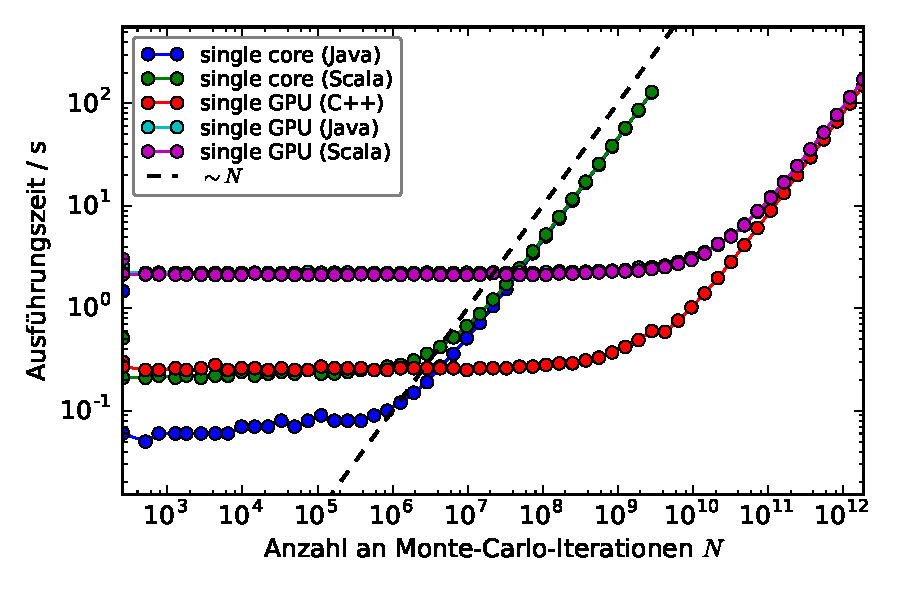
\includegraphics[width=0.8\linewidth]{benchmarks-workload-scaling.pdf}
    % sagen:
    %   - benchmarkImpl.sh misst mittels 'time' Linuxshellbefehls
    %   - overhead ist riesig, für GPU vs CPU und für Java vs. C++ -> relativ große Probleme rentieren sich nur
    %   - Java wird für sehr große Probleme schneller als C++ -> Vorteil der automatischen Optimierungen durch die JVM durch Rootbeer! -> nächste Seite Profiler nur kurz erwähnen
\end{frame}

\begin{frame}
Profiling von Rootbeer ohne Spark mit dem NVIDIA Visual Profiler:
    srun -p gpu-interactive --nodes=1 --ntasks-per-node=1 --cpus-per-task=1 --gres=gpu:2 --time=1:30:00 --mem-per-cpu=6000 --x11=first nvvp
    Executable: /sw/global/tools/java/jdk1.7.0_25/bin/java
    Working Directory: ... ???
    Arguments: -jar ./MontePi.jar 2684354560
       -> works :3
 -> BILDER!
\end{frame}

\begin{frame}
    \frametitle{Spark+GPU strong scaling}
    % cd scaromare/MontePi
    % make -C multiNode/multiGpu/scala ${makeOpts[@]} MontePi.jar
    % ./benchmarkTaurusScaling.sh
\end{frame}

%%%%%%%%%%%%%%%%%%%%%%%%%%%%%%%%%%%%%%%%%%%%%%%%%%%%%%%%%%%%%%%%%%%%%%%%%%%%%%%%
\section{Zusammenfassung}
%%%%%%%%%%%%%%%%%%%%%%%%%%%%%%%%%%%%%%%%%%%%%%%%%%%%%%%%%%%%%%%%%%%%%%%%%%%%%%%%

\begin{frame}
	\frametitle{Zusammenfassung}
	\begin{itemize}
		\item ...
	\end{itemize}
\end{frame}

%\appendix

\end{document}
